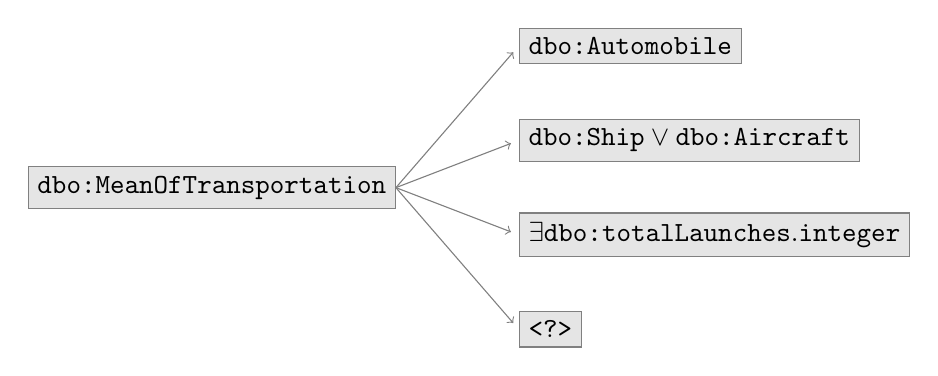
\begin{tikzpicture}[
  axiomnode/.style={fill=gray!20, draw=gray, anchor=west},
  axiomedge/.style={->, gray, shorten >=3pt},
]

\def\base{1.2};
\def\y{\base*1};
\def\x{\base*1.3};

\node[axiomnode] (a1) at (0, 3*\y) {\texttt{dbo:Automobile}};
\node[axiomnode] (a2) at (0, 2*\y) {$\texttt{dbo:Ship} \lor \texttt{dbo:Aircraft}$};
\node[axiomnode] (a3) at (0, \y) {$\exists \texttt{dbo:totalLaunches}.\texttt{integer}$};
\node[axiomnode] (a4) at (0, 0) {\texttt{<?>}};

\node[axiomnode, anchor=east] (root) at (-\x, 1.5*\y) {\texttt{dbo:MeanOfTransportation}};

\draw[axiomedge] (root.east) to (a1.west);
\draw[axiomedge] (root.east) to (a2.west);
\draw[axiomedge] (root.east) to (a3.west);
\draw[axiomedge] (root.east) to (a4.west);
\end{tikzpicture}